%%=============================================================================
%% LaTeX sjabloon voor bachelorproef, HoGent Bedrijf en Organisatie
%% Opleiding Toegepaste Informatica
%%=============================================================================

\documentclass[fleqn,a4paper,12pt]{book}

%%=============================================================================
%% LaTeX sjabloon voor de bachelorproef, HoGent Bedrijf en Organisatie
%% Opleiding toegepaste informatica
%%
%% Structuur en algemene vormgeving. Meestal hoef je hier niets te wijzigen.
%%
%% Vormgeving gebaseerd op "The Legrand Orange Book", version 2.0 (9/2/15)
%% door Mathias Legrand (legrand.mathias@gmail.com) met aanpassingen door
%% Vel (vel@latextemplates.com). Het oorspronkelijke template is te vinden op
%% http://www.LaTeXTemplates.com
%%
%% Aanpassingen voor HoGent toegepaste informatica: 
%%   Bert Van Vreckem <bert.vanvreckem@hogent.be>
%% Licentie: 
%%   CC BY-NC-SA 3.0 (http://creativecommons.org/licenses/by-nc-sa/3.0/)
%%=============================================================================

%%-----------------------------------------------------------------------------
%% Packages
%%-----------------------------------------------------------------------------

\usepackage[top=3cm,bottom=3cm,left=3cm,right=3cm,headsep=10pt,a4paper]{geometry} % Page margins
\usepackage[utf8]{inputenc}  % Accenten gebruiken in tekst (vb. é ipv \'e)
\usepackage{amsfonts}        % AMS math packages: extra wiskundige
\usepackage{amsmath}         %   symbolen (o.a. getallen-
\usepackage{amssymb}         %   verzamelingen N, R, Z, Q, etc.)
\usepackage[english,dutch]{babel}    % Taalinstellingen: woordsplitsingen,
                             %  commando's voor speciale karakters
                             %  ("dutch" voor NL)
\usepackage{iflang}
\usepackage{eurosym}         % Euro-symbool €
\usepackage{geometry}
\usepackage{graphicx}        % Invoegen van tekeningen
\graphicspath{{img/}}       % Specifies the directory where pictures are stored
\usepackage{tikz}            % Required for drawing custom shapes
\usepackage[pdftex,bookmarks=true]{hyperref}
                             % PDF krijgt klikbare links & verwijzingen,
                             %  inhoudstafel
\usepackage{enumitem}        % Customize lists
\setlist{nolistsep}         % Reduce spacing between list items
\usepackage{listings}        % Broncode mooi opmaken
\usepackage{multirow}        % Tekst over verschillende cellen in tabellen
\usepackage{rotating}        % Tabellen en figuren roteren

\usepackage{booktabs}        % Required for nicer horizontal rules in tables

\usepackage{xcolor}          % Required for specifying colors by name
\definecolor{maincolor}{RGB}{0,147,208} % Define the main color used for 
                             % highlighting throughout the book
                             % 0, 147, 208 = officiële kleur HoGent FBO

% Paragraph style: no indent, add space between paragraphs
\setlength{\parindent}{0em}
\setlength{\parskip}{1em}

\usepackage{etoolbox}
\usepackage{titling} % Macros for title, author, etc
\usepackage{lipsum}          % Voor vultekst (lorem ipsum)

%----------------------------------------------------------------------------------------
%	FONTS
%----------------------------------------------------------------------------------------

\usepackage{avant} % Use the Avantgarde font for headings
%\usepackage{times} % Use the Times font for headings
\usepackage{mathptmx} % Use the Adobe Times Roman as the default text font together with math symbols from the Sym­bol, Chancery and Com­puter Modern fonts

\usepackage{microtype} % Slightly tweak font spacing for aesthetics
\usepackage[utf8]{inputenc} % Required for including letters with accents
\usepackage[T1]{fontenc} % Use 8-bit encoding that has 256 glyphs

%------------------------------------------------------------------------------
%	TITLE PAGE
%------------------------------------------------------------------------------

\newcommand{\inserttitlepage}{%
\begin{titlepage}
  \newgeometry{top=2cm,bottom=1.5cm,left=1.5cm,right=1.5cm}
  \begin{center}

    \begingroup
    \rmfamily
    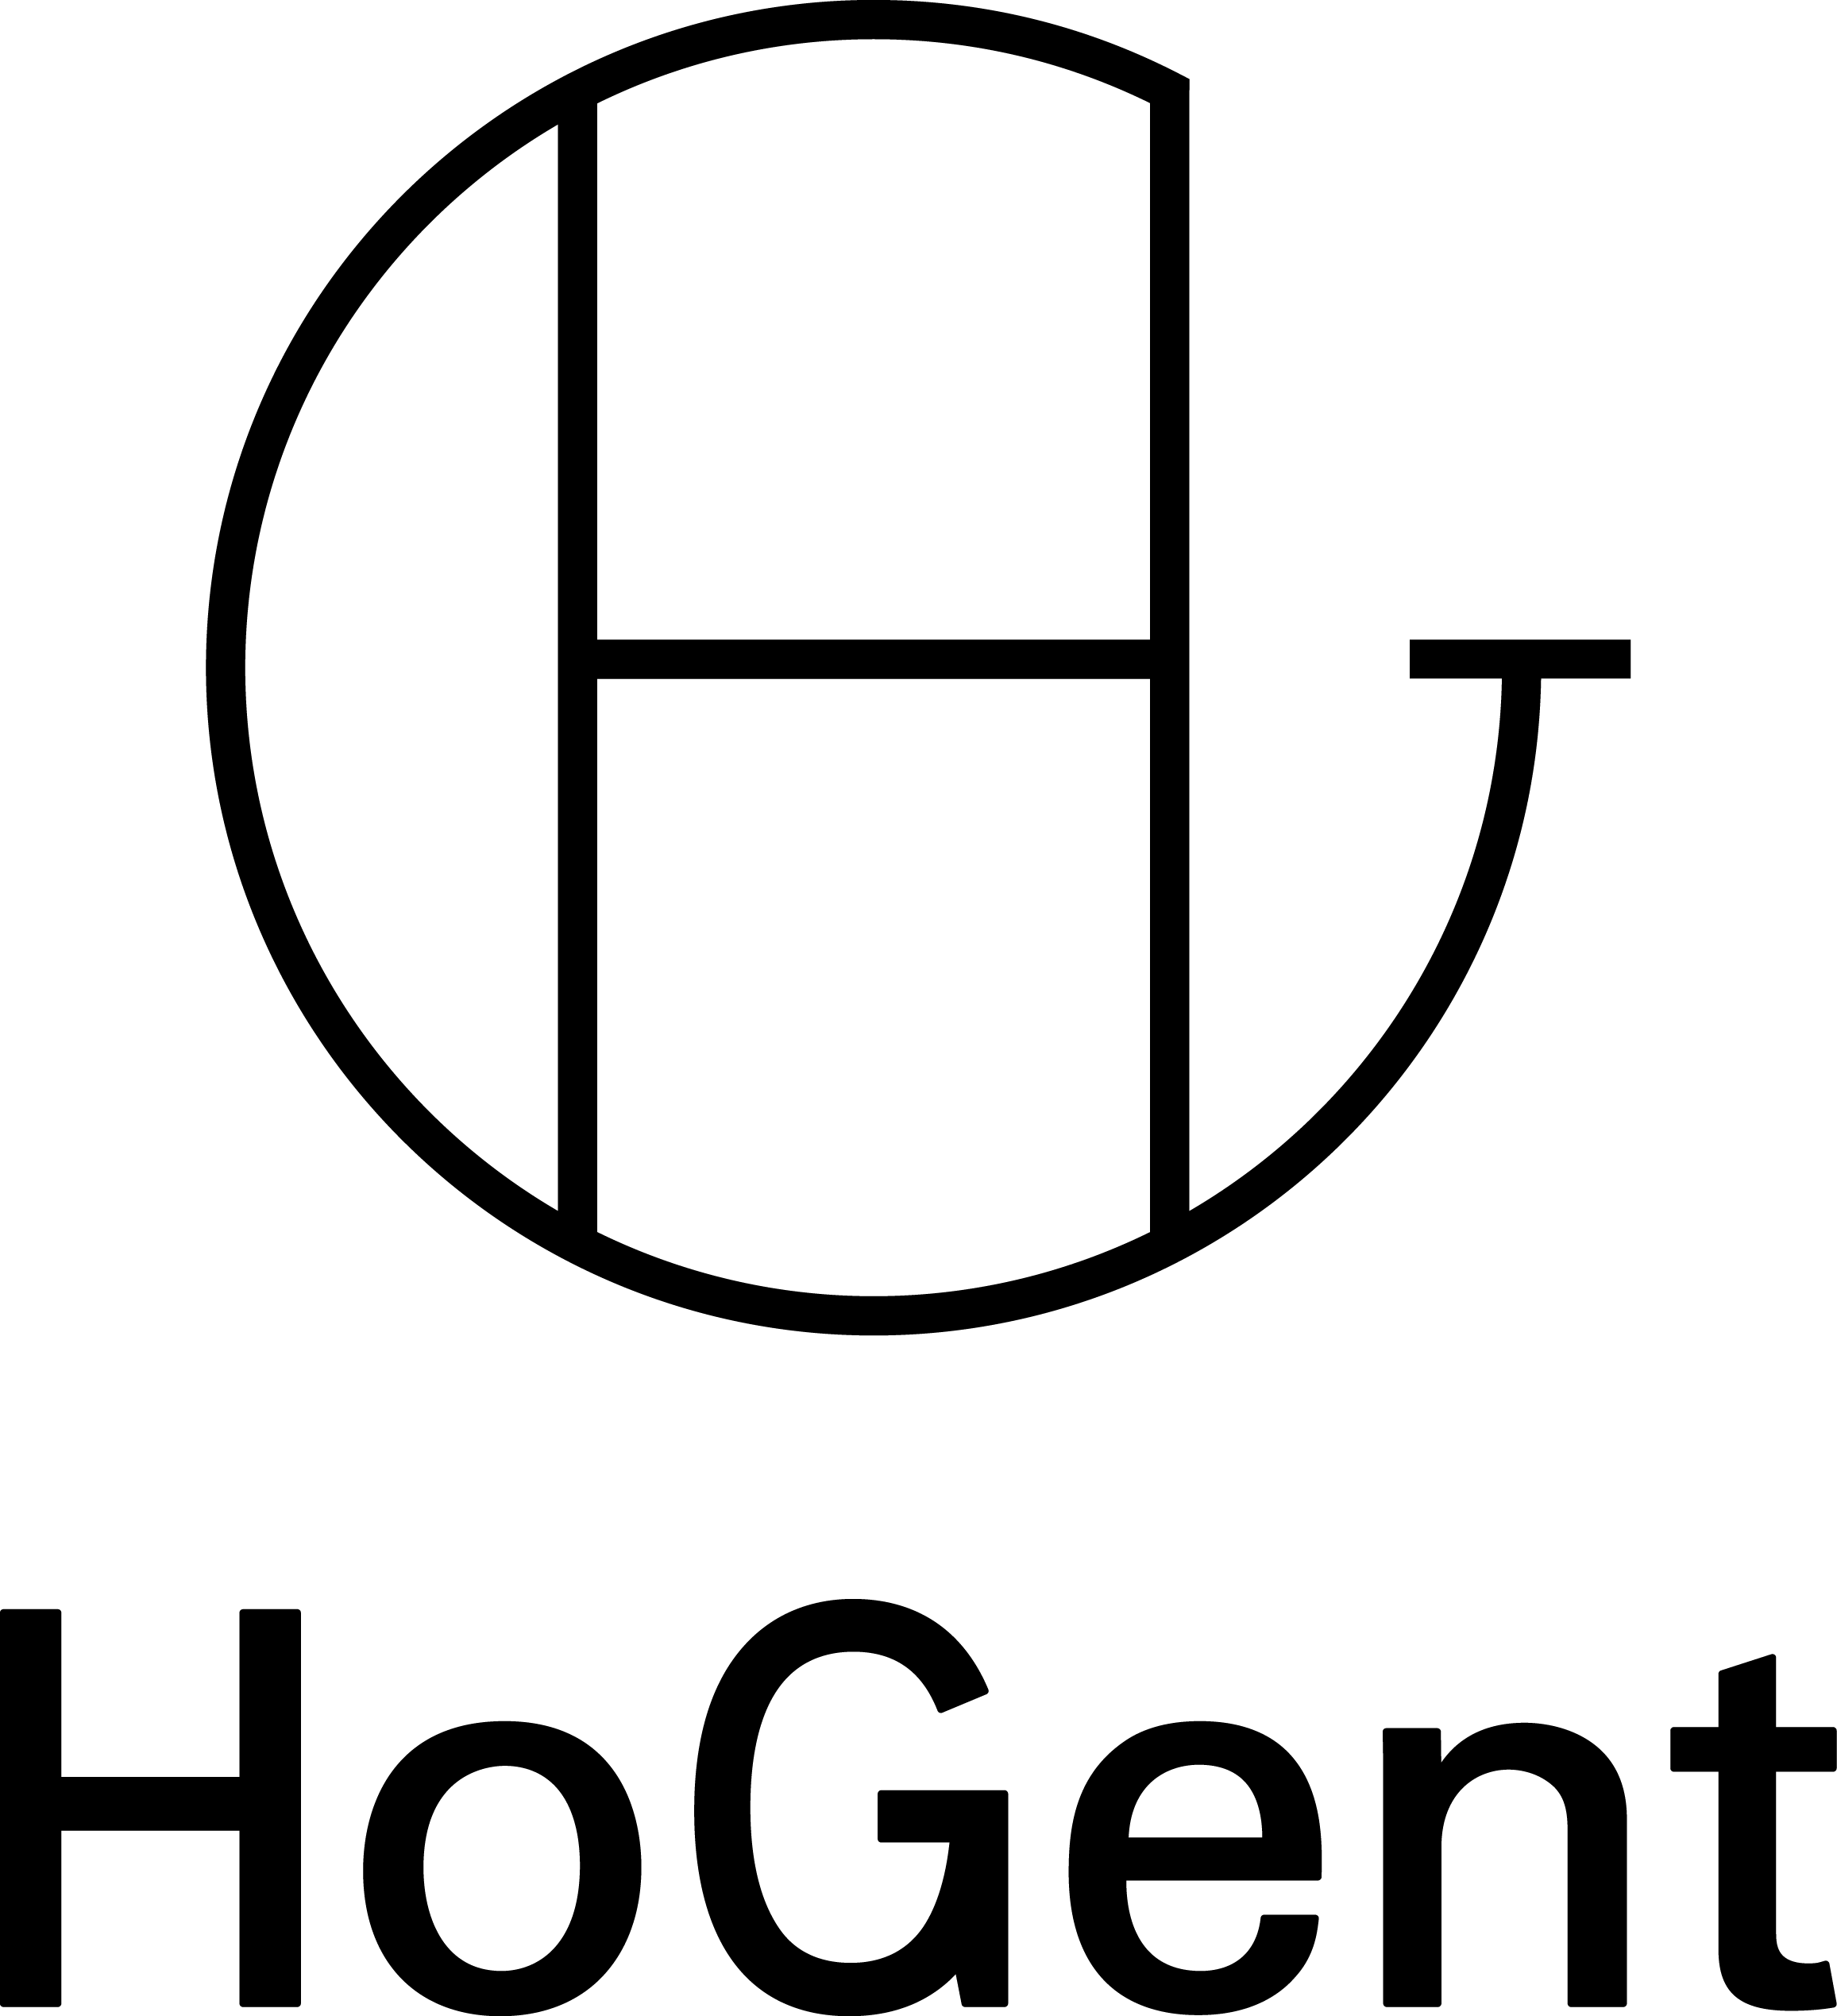
\includegraphics[width=2.5cm]{img/HG-beeldmerk-woordmerk}\\[.5cm]
    Faculteit Bedrijf en Organisatie\\[3cm]
    \titel
    \vfill
    \student\\[3.5cm]
    Scriptie voorgedragen tot het bekomen van de graad van\\professionele bachelor in de toegepaste informatica\\[2cm]
    Promotor:\\
    \promotor\\
    \ifdefempty{\copromotor}{\vspace{2.5cm}}{Co-promotor:\\\copromotor\\[2.5cm]}
    Instelling: \instelling\\[.5cm]
    Academiejaar: \academiejaar\\[.5cm]
    \ifcase \examenperiode \or Eerste \or Tweede \else Derde \fi examenperiode
    \endgroup

  \end{center}
  \restoregeometry
\end{titlepage}
  \emptypage
\begin{titlepage}
  \newgeometry{top=5.35cm,bottom=1.5cm,left=1.5cm,right=1.5cm}
  \begin{center}

    \begingroup
    \rmfamily
    \IfLanguageName{dutch}{Faculteit Bedrijf en Organisatie}{Faculty of Business and Information Management}\\[3cm]
    \titel
    \vfill
    \student\\[3.5cm]
    \IfLanguageName{dutch}{Scriptie voorgedragen tot het bekomen van de graad van\\professionele bachelor in de toegepaste informatica}{Thesis submitted in partial fulfilment of the requirements for the degree of\\professional bachelor of applied computer science}\\[2cm]
    Promotor:\\
    \promotor\\
    \ifdefempty{\copromotor}{\vspace{2.5cm}}{Co-promotor:\\\copromotor\\[2.5cm]}
    \IfLanguageName{dutch}{Instelling}{Institution}: \instelling\\[.5cm]
    \IfLanguageName{dutch}{Academiejaar}{Academic year}: \academiejaar\\[.5cm]
    \IfLanguageName{dutch}{%
    \ifcase \examenperiode \or Eerste \or Tweede \else Derde \fi examenperiode}{%
    \ifcase \examenperiode \or First \or Second \else Third \fi examination period}
    \endgroup

  \end{center}
  \restoregeometry
\end{titlepage}
}

%----------------------------------------------------------------------------------------
%	BIBLIOGRAPHY AND INDEX
%----------------------------------------------------------------------------------------

\usepackage[style=apa,backend=biber]{biblatex}
\usepackage{csquotes}
\DeclareLanguageMapping{dutch}{dutch-apa}
\addbibresource{bachproef-tin.bib} % BibTeX bibliography file
\addbibresource{../voorstel/voorstel.bib}
\defbibheading{bibempty}{}

\usepackage{calc} % For simpler calculation - used for spacing the index letter headings correctly
\usepackage{makeidx} % Required to make an index
\makeindex % Tells LaTeX to create the files required for indexing

%----------------------------------------------------------------------------------------
%	MAIN TABLE OF CONTENTS
%----------------------------------------------------------------------------------------

\usepackage{titletoc} % Required for manipulating the table of contents

\contentsmargin{0cm} % Removes the default margin

% Part text styling
\titlecontents{part}[0cm]
{\addvspace{20pt}\centering\large\bfseries}
{}
{}
{}

% Chapter text styling
\titlecontents{chapter}[1.25cm] % Indentation
{\addvspace{12pt}\large\sffamily\bfseries} % Spacing and font options for chapters
{\color{maincolor!60}\contentslabel[\Large\thecontentslabel]{1.25cm}\color{maincolor}} % Chapter number
{\color{maincolor}}
{\color{maincolor!60}\normalsize\;\titlerule*[.5pc]{.}\;\thecontentspage} % Page number

% Section text styling
\titlecontents{section}[1.25cm] % Indentation
{\addvspace{3pt}\sffamily\bfseries} % Spacing and font options for sections
{\contentslabel[\thecontentslabel]{1.25cm}} % Section number
{}
{\hfill\color{black}\thecontentspage} % Page number
[]

% Subsection text styling
\titlecontents{subsection}[1.25cm] % Indentation
{\addvspace{1pt}\sffamily\small} % Spacing and font options for subsections
{\contentslabel[\thecontentslabel]{1.25cm}} % Subsection number
{}
{\ \titlerule*[.5pc]{.}\;\thecontentspage} % Page number
[]

% List of figures
\titlecontents{figure}[0em]
{\addvspace{-5pt}\sffamily}
{\thecontentslabel\hspace*{1em}}
{}
{\ \titlerule*[.5pc]{.}\;\thecontentspage}
[]

% List of tables
\titlecontents{table}[0em]
{\addvspace{-5pt}\sffamily}
{\thecontentslabel\hspace*{1em}}
{}
{\ \titlerule*[.5pc]{.}\;\thecontentspage}
[]

%----------------------------------------------------------------------------------------
%	MINI TABLE OF CONTENTS IN PART HEADS
%----------------------------------------------------------------------------------------

% Chapter text styling
\titlecontents{lchapter}[0em] % Indenting
{\addvspace{15pt}\large\sffamily\bfseries} % Spacing and font options for chapters
{\color{maincolor}\contentslabel[\Large\thecontentslabel]{1.25cm}\color{maincolor}} % Chapter number
{}
{\color{maincolor}\normalsize\sffamily\bfseries\;\titlerule*[.5pc]{.}\;\thecontentspage} % Page number

% Section text styling
\titlecontents{lsection}[0em] % Indenting
{\sffamily\small} % Spacing and font options for sections
{\contentslabel[\thecontentslabel]{1.25cm}} % Section number
{}
{}

% Subsection text styling
\titlecontents{lsubsection}[.5em] % Indentation
{\normalfont\footnotesize\sffamily} % Font settings
{}
{}
{}

%----------------------------------------------------------------------------------------
%	PAGE HEADERS
%----------------------------------------------------------------------------------------

\usepackage{fancyhdr} % Required for header and footer configuration

\pagestyle{fancy}
\renewcommand{\chaptermark}[1]{\markboth{\sffamily\normalsize\bfseries\chaptername\ \thechapter.\ #1}{}} % Chapter text font settings
\renewcommand{\sectionmark}[1]{\markright{\sffamily\normalsize\thesection\hspace{5pt}#1}{}} % Section text font settings
\fancyhf{} \fancyhead[LE,RO]{\sffamily\normalsize\thepage} % Font setting for the page number in the header
\fancyhead[LO]{\rightmark} % Print the nearest section name on the left side of odd pages
\fancyhead[RE]{\leftmark} % Print the current chapter name on the right side of even pages
\renewcommand{\headrulewidth}{0.5pt} % Width of the rule under the header
\addtolength{\headheight}{2.5pt} % Increase the spacing around the header slightly
\renewcommand{\footrulewidth}{0pt} % Removes the rule in the footer
\fancypagestyle{plain}{\fancyhead{}\renewcommand{\headrulewidth}{0pt}} % Style for when a plain pagestyle is specified

% Removes the header from odd empty pages at the end of chapters
\makeatletter
\renewcommand{\cleardoublepage}{
\clearpage\ifodd\c@page\else
\hbox{}
\vspace*{\fill}
\thispagestyle{empty}
\newpage
\fi}

%----------------------------------------------------------------------------------------
%	THEOREM STYLES
%----------------------------------------------------------------------------------------

\usepackage{amsmath,amsfonts,amssymb,amsthm} % For math equations, theorems, symbols, etc

\newcommand{\intoo}[2]{\mathopen{]}#1\,;#2\mathclose{[}}
\newcommand{\ud}{\mathop{\mathrm{{}d}}\mathopen{}}
\newcommand{\intff}[2]{\mathopen{[}#1\,;#2\mathclose{]}}
\newtheorem{notation}{Notation}[chapter]

% Boxed/framed environments
\newtheoremstyle{maincolornumbox}% % Theorem style name
{0pt}% Space above
{0pt}% Space below
{\normalfont}% % Body font
{}% Indent amount
{\small\bf\sffamily\color{maincolor}}% % Theorem head font
{\;}% Punctuation after theorem head
{0.25em}% Space after theorem head
{\small\sffamily\color{maincolor}\thmname{#1}\nobreakspace\thmnumber{\@ifnotempty{#1}{}\@upn{#2}}% Theorem text (e.g. Theorem 2.1)
\thmnote{\nobreakspace\the\thm@notefont\sffamily\bfseries\color{black}---\nobreakspace#3.}} % Optional theorem note
\renewcommand{\qedsymbol}{$\blacksquare$}% Optional qed square

\newtheoremstyle{blacknumex}% Theorem style name
{5pt}% Space above
{5pt}% Space below
{\normalfont}% Body font
{} % Indent amount
{\small\bf\sffamily}% Theorem head font
{\;}% Punctuation after theorem head
{0.25em}% Space after theorem head
{\small\sffamily{\tiny\ensuremath{\blacksquare}}\nobreakspace\thmname{#1}\nobreakspace\thmnumber{\@ifnotempty{#1}{}\@upn{#2}}% Theorem text (e.g. Theorem 2.1)
\thmnote{\nobreakspace\the\thm@notefont\sffamily\bfseries---\nobreakspace#3.}}% Optional theorem note

\newtheoremstyle{blacknumbox} % Theorem style name
{0pt}% Space above
{0pt}% Space below
{\normalfont}% Body font
{}% Indent amount
{\small\bf\sffamily}% Theorem head font
{\;}% Punctuation after theorem head
{0.25em}% Space after theorem head
{\small\sffamily\thmname{#1}\nobreakspace\thmnumber{\@ifnotempty{#1}{}\@upn{#2}}% Theorem text (e.g. Theorem 2.1)
\thmnote{\nobreakspace\the\thm@notefont\sffamily\bfseries---\nobreakspace#3.}}% Optional theorem note

% Non-boxed/non-framed environments
\newtheoremstyle{maincolornum}% % Theorem style name
{5pt}% Space above
{5pt}% Space below
{\normalfont}% % Body font
{}% Indent amount
{\small\bf\sffamily\color{maincolor}}% % Theorem head font
{\;}% Punctuation after theorem head
{0.25em}% Space after theorem head
{\small\sffamily\color{maincolor}\thmname{#1}\nobreakspace\thmnumber{\@ifnotempty{#1}{}\@upn{#2}}% Theorem text (e.g. Theorem 2.1)
\thmnote{\nobreakspace\the\thm@notefont\sffamily\bfseries\color{black}---\nobreakspace#3.}} % Optional theorem note
\renewcommand{\qedsymbol}{$\blacksquare$}% Optional qed square
\makeatother

% Defines the theorem text style for each type of theorem to one of the three styles above
\newcounter{dummy}
\numberwithin{dummy}{section}
\theoremstyle{maincolornumbox}
\newtheorem{theoremeT}[dummy]{Theorem}
\newtheorem{problem}{Problem}[chapter]
\newtheorem{exerciseT}{Exercise}[chapter]
\theoremstyle{blacknumex}
\newtheorem{exampleT}{Example}[chapter]
\theoremstyle{blacknumbox}
\newtheorem{vocabulary}{Vocabulary}[chapter]
\newtheorem{definitionT}{Definition}[section]
\newtheorem{corollaryT}[dummy]{Corollary}
\theoremstyle{maincolornum}
\newtheorem{proposition}[dummy]{Proposition}

%----------------------------------------------------------------------------------------
%	DEFINITION OF COLORED BOXES
%----------------------------------------------------------------------------------------

\RequirePackage[framemethod=default]{mdframed} % Required for creating the theorem, definition, exercise and corollary boxes

% Theorem box
\newmdenv[skipabove=7pt,
skipbelow=7pt,
backgroundcolor=black!5,
linecolor=maincolor,
innerleftmargin=5pt,
innerrightmargin=5pt,
innertopmargin=5pt,
leftmargin=0cm,
rightmargin=0cm,
innerbottommargin=5pt]{tBox}

% Exercise box
\newmdenv[skipabove=7pt,
skipbelow=7pt,
rightline=false,
leftline=true,
topline=false,
bottomline=false,
backgroundcolor=maincolor!10,
linecolor=maincolor,
innerleftmargin=5pt,
innerrightmargin=5pt,
innertopmargin=5pt,
innerbottommargin=5pt,
leftmargin=0cm,
rightmargin=0cm,
linewidth=4pt]{eBox}

% Definition box
\newmdenv[skipabove=7pt,
skipbelow=7pt,
rightline=false,
leftline=true,
topline=false,
bottomline=false,
linecolor=maincolor,
innerleftmargin=5pt,
innerrightmargin=5pt,
innertopmargin=0pt,
leftmargin=0cm,
rightmargin=0cm,
linewidth=4pt,
innerbottommargin=0pt]{dBox}

% Corollary box
\newmdenv[skipabove=7pt,
skipbelow=7pt,
rightline=false,
leftline=true,
topline=false,
bottomline=false,
linecolor=gray,
backgroundcolor=black!5,
innerleftmargin=5pt,
innerrightmargin=5pt,
innertopmargin=5pt,
leftmargin=0cm,
rightmargin=0cm,
linewidth=4pt,
innerbottommargin=5pt]{cBox}

% Creates an environment for each type of theorem and assigns it a theorem text style from the "Theorem Styles" section above and a colored box from above
\newenvironment{theorem}{\begin{tBox}\begin{theoremeT}}{\end{theoremeT}\end{tBox}}
\newenvironment{exercise}{\begin{eBox}\begin{exerciseT}}{\hfill{\color{maincolor}\tiny\ensuremath{\blacksquare}}\end{exerciseT}\end{eBox}}
\newenvironment{definition}{\begin{dBox}\begin{definitionT}}{\end{definitionT}\end{dBox}}
\newenvironment{example}{\begin{exampleT}}{\hfill{\tiny\ensuremath{\blacksquare}}\end{exampleT}}
\newenvironment{corollary}{\begin{cBox}\begin{corollaryT}}{\end{corollaryT}\end{cBox}}

%----------------------------------------------------------------------------------------
%	REMARK ENVIRONMENT
%----------------------------------------------------------------------------------------

\newenvironment{remark}{\par\vspace{10pt}\small % Vertical white space above the remark and smaller font size
\begin{list}{}{
\leftmargin=35pt % Indentation on the left
\rightmargin=25pt}\item\ignorespaces % Indentation on the right
\makebox[-2.5pt]{\begin{tikzpicture}[overlay]
\node[draw=maincolor!60,line width=1pt,circle,fill=maincolor!25,font=\sffamily\bfseries,inner sep=2pt,outer sep=0pt] at (-15pt,0pt){\textcolor{maincolor}{R}};\end{tikzpicture}} % Orange R in a circle
\advance\baselineskip -1pt}{\end{list}\vskip5pt} % Tighter line spacing and white space after remark

%----------------------------------------------------------------------------------------
%	SECTION NUMBERING IN THE MARGIN
%----------------------------------------------------------------------------------------

\makeatletter
\renewcommand{\@seccntformat}[1]{\llap{\textcolor{maincolor}{\csname the#1\endcsname}\hspace{1em}}}
\renewcommand{\section}{\@startsection{section}{1}{\z@}
{-4ex \@plus -1ex \@minus -.4ex}
{1ex \@plus.2ex }
{\normalfont\large\sffamily\bfseries}}
\renewcommand{\subsection}{\@startsection {subsection}{2}{\z@}
{-3ex \@plus -0.1ex \@minus -.4ex}
{0.5ex \@plus.2ex }
{\normalfont\sffamily\bfseries}}
\renewcommand{\subsubsection}{\@startsection {subsubsection}{3}{\z@}
{-2ex \@plus -0.1ex \@minus -.2ex}
{.2ex \@plus.2ex }
{\normalfont\small\sffamily\bfseries}}
\renewcommand\paragraph{\@startsection{paragraph}{4}{\z@}
{-2ex \@plus-.2ex \@minus .2ex}
{.1ex}
{\normalfont\small\sffamily\bfseries}}

%----------------------------------------------------------------------------------------
%	PART HEADINGS
%----------------------------------------------------------------------------------------

% numbered part in the table of contents
\newcommand{\@mypartnumtocformat}[2]{%
\setlength\fboxsep{0pt}%
\noindent\colorbox{maincolor!20}{\strut\parbox[c][.7cm]{\ecart}{\color{maincolor!70}\Large\sffamily\bfseries\centering#1}}\hskip\esp\colorbox{maincolor!40}{\strut\parbox[c][.7cm]{\linewidth-\ecart-\esp}{\Large\sffamily\centering#2}}}%
%%%%%%%%%%%%%%%%%%%%%%%%%%%%%%%%%%
% unnumbered part in the table of contents
\newcommand{\@myparttocformat}[1]{%
\setlength\fboxsep{0pt}%
\noindent\colorbox{maincolor!40}{\strut\parbox[c][.7cm]{\linewidth}{\Large\sffamily\centering#1}}}%
%%%%%%%%%%%%%%%%%%%%%%%%%%%%%%%%%%
\newlength\esp
\setlength\esp{4pt}
\newlength\ecart
\setlength\ecart{1.2cm-\esp}
\newcommand{\thepartimage}{}%
\newcommand{\partimage}[1]{\renewcommand{\thepartimage}{#1}}%
\def\@part[#1]#2{%
\ifnum \c@secnumdepth >-2\relax%
\refstepcounter{part}%
\addcontentsline{toc}{part}{\texorpdfstring{\protect\@mypartnumtocformat{\thepart}{#1}}{\partname~\thepart\ ---\ #1}}
\else%
\addcontentsline{toc}{part}{\texorpdfstring{\protect\@myparttocformat{#1}}{#1}}%
\fi%
\startcontents%
\markboth{}{}%
{\thispagestyle{empty}%
\begin{tikzpicture}[remember picture,overlay]%
\node at (current page.north west){\begin{tikzpicture}[remember picture,overlay]%
\fill[maincolor!20](0cm,0cm) rectangle (\paperwidth,-\paperheight);
\node[anchor=north] at (4cm,-3.25cm){\color{maincolor!40}\fontsize{220}{100}\sffamily\bfseries\@Roman\c@part};
\node[anchor=south east] at (\paperwidth-1cm,-\paperheight+1cm){\parbox[t][][t]{8.5cm}{
\printcontents{l}{0}{\setcounter{tocdepth}{1}}%
}};
\node[anchor=north east] at (\paperwidth-1.5cm,-3.25cm){\parbox[t][][t]{15cm}{\strut\raggedleft\color{white}\fontsize{30}{30}\sffamily\bfseries#2}};
\end{tikzpicture}};
\end{tikzpicture}}%
\@endpart}
\def\@spart#1{%
\startcontents%
\phantomsection
{\thispagestyle{empty}%
\begin{tikzpicture}[remember picture,overlay]%
\node at (current page.north west){\begin{tikzpicture}[remember picture,overlay]%
\fill[maincolor!20](0cm,0cm) rectangle (\paperwidth,-\paperheight);
\node[anchor=north east] at (\paperwidth-1.5cm,-3.25cm){\parbox[t][][t]{15cm}{\strut\raggedleft\color{white}\fontsize{30}{30}\sffamily\bfseries#1}};
\end{tikzpicture}};
\end{tikzpicture}}
\addcontentsline{toc}{part}{\texorpdfstring{%
\setlength\fboxsep{0pt}%
\noindent\protect\colorbox{maincolor!40}{\strut\protect\parbox[c][.7cm]{\linewidth}{\Large\sffamily\protect\centering #1\quad\mbox{}}}}{#1}}%
\@endpart}
\def\@endpart{\vfil\newpage
\if@twoside
\if@openright
\null
\thispagestyle{empty}%
\newpage
\fi
\fi
\if@tempswa
\twocolumn
\fi}

%----------------------------------------------------------------------------------------
%	CHAPTER HEADINGS
%----------------------------------------------------------------------------------------

% A switch to conditionally include a picture, implemented by  Christian Hupfer
\newif\ifusechapterimage
\usechapterimagetrue
\newcommand{\thechapterimage}{}%
\newcommand{\chapterimage}[1]{\ifusechapterimage\renewcommand{\thechapterimage}{#1}\fi}%
\def\@makechapterhead#1{%
{\parindent \z@ \raggedright \normalfont
\ifnum \c@secnumdepth >\m@ne
\if@mainmatter
\begin{tikzpicture}[remember picture,overlay]
\node at (current page.north west)
{\begin{tikzpicture}[remember picture,overlay]
\node[anchor=north west,inner sep=0pt] at (0,0) {\ifusechapterimage\includegraphics[width=\paperwidth]{\thechapterimage}\fi};
\draw[anchor=west] (\Gm@lmargin,-9cm) node [line width=2pt,rounded corners=15pt,draw=maincolor,fill=white,fill opacity=0.5,inner sep=15pt]{\strut\makebox[22cm]{}};
\draw[anchor=west] (\Gm@lmargin+.3cm,-9cm) node {\huge\sffamily\bfseries\color{black}\thechapter. #1\strut};
\end{tikzpicture}};
\end{tikzpicture}
\else
\begin{tikzpicture}[remember picture,overlay]
\node at (current page.north west)
{\begin{tikzpicture}[remember picture,overlay]
\node[anchor=north west,inner sep=0pt] at (0,0) {\ifusechapterimage\includegraphics[width=\paperwidth]{\thechapterimage}\fi};
\draw[anchor=west] (\Gm@lmargin,-9cm) node [line width=2pt,rounded corners=15pt,draw=maincolor,fill=white,fill opacity=0.5,inner sep=15pt]{\strut\makebox[22cm]{}};
\draw[anchor=west] (\Gm@lmargin+.3cm,-9cm) node {\huge\sffamily\bfseries\color{black}#1\strut};
\end{tikzpicture}};
\end{tikzpicture}
\fi\fi\par\vspace*{270\p@}}}

%-------------------------------------------

\def\@makeschapterhead#1{%
\begin{tikzpicture}[remember picture,overlay]
\node at (current page.north west)
{\begin{tikzpicture}[remember picture,overlay]
\node[anchor=north west,inner sep=0pt] at (0,0) {\ifusechapterimage\includegraphics[width=\paperwidth]{\thechapterimage}\fi};
\draw[anchor=west] (\Gm@lmargin,-9cm) node [line width=2pt,rounded corners=15pt,draw=maincolor,fill=white,fill opacity=0.5,inner sep=15pt]{\strut\makebox[22cm]{}};
\draw[anchor=west] (\Gm@lmargin+.3cm,-9cm) node {\huge\sffamily\bfseries\color{black}#1\strut};
\end{tikzpicture}};
\end{tikzpicture}
\par\vspace*{270\p@}}
\makeatother

%----------------------------------------------------------------------------------------
%	HYPERLINKS IN THE DOCUMENTS
%----------------------------------------------------------------------------------------

\usepackage{hyperref}
\hypersetup{hidelinks,backref=true,pagebackref=true,hyperindex=true,colorlinks=false,breaklinks=true,urlcolor= maincolor,bookmarks=true,bookmarksopen=false,pdftitle={Title},pdfauthor={Author}}
\usepackage{bookmark}
\bookmarksetup{
open,
numbered,
addtohook={%
\ifnum\bookmarkget{level}=0 % chapter
\bookmarksetup{bold}%
\fi
\ifnum\bookmarkget{level}=-1 % part
\bookmarksetup{color=maincolor,bold}%
\fi
}
}

%----------------------------------------------------------------------------------------
%	Java source code
%----------------------------------------------------------------------------------------

% Commando voor invoegen Java-broncodebestanden (dank aan Niels Corneille)
% Gebruik:
%   \codefragment{source/MijnKlasse.java}{Uitleg bij de code}
%
% Je kan dit aanpassen aan de taal die je zelf het meeste gebruikt in je
% bachelorproef.
\newcommand{\codefragment}[2]{ \lstset{%
  language=java,
  breaklines=true,
  float=th,
  caption={#2},
  basicstyle=\scriptsize,
  frame=single,
  extendedchars=\true
}
\lstinputlisting{#1}}

% Leeg blad
\newcommand{\emptypage}{%
\newpage
\thispagestyle{empty}
\mbox{}
\newpage
}


%%---------- Documenteigenschappen --------------------------------------------
%% TODO: Vul dit aan met je eigen info:

% Je eigen naam
\newcommand{\student}{Stephan Heirbaut}

% De naam van je promotor (lector van de opleiding)
\newcommand{\promotor}{Steven Vermeulen}

% De naam van je co-promotor. Als je promotor ook je opdrachtgever is en je
% dus ook inhoudelijk begeleidt (en enkel dan!), mag je dit leeg laten.
\newcommand{\copromotor}{Gert Schepens}

% Indien je bachelorproef in opdracht van/in samenwerking met een bedrijf of
% externe organisatie geschreven is, geef je hier de naam. Zoniet laat je dit
% zoals het is.
\newcommand{\instelling}{---}

% De titel van het rapport/bachelorproef
\newcommand{\titel}{Docker for Windows}

% Datum van indienen (gebruik telkens de deadline, ook al geef je eerder af)
\newcommand{\datum}{28 mei 2018}

% Academiejaar
\newcommand{\academiejaar}{2017-2018}

% Examenperiode
%  - 1e semester = 1e examenperiode => 1
%  - 2e semester = 2e examenperiode => 2
%  - tweede zit  = 3e examenperiode => 3
\newcommand{\examenperiode}{2}

%%=============================================================================
%% Inhoud document
%%=============================================================================

\begin{document}

%---------- Taalselectie ------------------------------------------------------
%% Als je je bachelorproef in het Engels schrijft, haal dan onderstaande regel
%% uit commentaar. Let op: de tekst op de voorkaft blijft in het Nederlands, en
%% dat is ook de bedoeling!
%\selectlanguage{english}

%---------- Titelblad ---------------------------------------------------------
\inserttitlepage

%---------- Samenvatting, voorwoord -------------------------------------------
\usechapterimagefalse
%%=============================================================================
%% Samenvatting
%%=============================================================================

%% TODO: De "abstract" of samenvatting is een kernachtige (~ 1 blz. voor een
%% thesis) synthese van het document.
%%
%% Deze aspecten moeten zeker aan bod komen:
%% - Context: waarom is dit werk belangrijk?
%% - Nood: waarom moest dit onderzocht worden?
%% - Taak: wat heb je precies gedaan?
%% - Object: wat staat in dit document geschreven?
%% - Resultaat: wat was het resultaat?
%% - Conclusie: wat is/zijn de belangrijkste conclusie(s)?
%% - Perspectief: blijven er nog vragen open die in de toekomst nog kunnen
%%    onderzocht worden? Wat is een mogelijk vervolg voor jouw onderzoek?
%%
%% LET OP! Een samenvatting is GEEN voorwoord!

%%---------- Nederlandse samenvatting -----------------------------------------
%%
%% TODO: Als je je bachelorproef in het Engels schrijft, moet je eerst een
%% Nederlandse samenvatting invoegen. Haal daarvoor onderstaande code uit
%% commentaar.
%% Wie zijn bachelorproef in het Nederlands schrijft, kan dit negeren en heel
%% deze sectie verwijderen.

\IfLanguageName{english}{%
\selectlanguage{dutch}
\chapter*{Samenvatting}
\lipsum[1-4]
\selectlanguage{english}
}{}

%%---------- Samenvatting -----------------------------------------------------
%%
%% De samenvatting in de hoofdtaal van het document

\chapter*{\IfLanguageName{dutch}{Samenvatting}{Abstract}}

Docker for Windows Server 2016 is uit beta gekomen op 22 februari 2017. Maar, ondanks het feit dat dit platform nu al een ruime tijd beschikbaar is, heeft het nog steeds geen tractie gevonden bij DevOps-teams. Dit ondanks het feit dat dit een krachtige tool kan zijn voor organisaties die ook Microsoft Certified Partners willen zijn. In een notendop, er zal dus gekeken worden of Docker for Windows Server 2016 een goed alternatief is voor het draaien van Docker in een Linux omgeving. Om dit op een methodologische manier uit te testen zal er vertrokken worden van een standaard Windows Server 2016 en CentOS 7.4 installatie waarop Docker geïnstalleerd zal worden. Waarna beide omgevingen getest zullen door middel van performatie-, integratie- en beveiligingstesten, om zo een vergelijking te maken van beide omgevingen. Daarbovenop zal ook de documentatie voor beide platformen bekeken worden op vlak van compleetheid.
\par
De verwachting is dat het verschil tussen beide systemen minimaal zal zijn, waarbij de CentOS server beter zal presteren op vlak van beveiliging en performantie, en dat Windows Server 2016 beter zal presteren op vlak van integratie. De documentatie voor CentOS zal ook meer compleet zijn, maar dat zowel Windows als Docker een grote inhaalbeweging aan het maken zijn.
\par
Verdere vragen die men hierna nog zou kunnen stellen zijn:
\begin{itemize}[noitemsep]
	\item Hoe goed scoren beide op vlak van user-friendliness?
	\item Hoe goed ondersteunen beide Cloud platforms?
	\item Hoe stabiel draaien beide omgevingen?
\end{itemize}
%%=============================================================================
%% Voorwoord
%%=============================================================================

\chapter*{Voorwoord}
\label{ch:voorwoord}

%% TODO:
%% Het voorwoord is het enige deel van de bachelorproef waar je vanuit je
%% eigen standpunt (``ik-vorm'') mag schrijven. Je kan hier bv. motiveren
%% waarom jij het onderwerp wil bespreken.
%% Vergeet ook niet te bedanken wie je geholpen/gesteund/... heeft

%De eerste zinnen van het voorwoord vertellen waar het boek, de scriptie of het verslag inhoudelijk over gaat.
%Daarna volgt de aanleiding tot het schrijven van het boek, de scriptie of het verslag.
%Vervolgens vertelt u uw ervaringen als schrijver van de geschreven tekst.
%U bedankt alle mensen die erbij betrokken waren en/of waar u mee heeft samengewerkt. Hierbij kunt u denken aan de vertaler, begeleider of proeflezer.
%Daarna bedankt u vrienden en familie voor de steun die zij u hebben gegeven tijdens het schrijven.
%Vervolgens ondertekent u het voorwoord met uw naam; het is tenslotte een persoonlijk stuk.
%U sluit af met de datum en de plaats.



%---------- Inhoudstafel ------------------------------------------------------
\pagestyle{empty} % No headers
\tableofcontents % Print the table of contents itself
\cleardoublepage % Forces the first chapter to start on an odd page so it's on the right
\pagestyle{fancy} % Print headers again

%---------- Lijst afkortingen, termen -----------------------------------------
%% Als je een lijst van afkortingen of termen wil toevoegen, dan hoort die
%% hier thuis. Gebruik bijvoorbeeld de ``glossaries'' package.

%%---------- Kern -------------------------------------------------------------

%%=============================================================================
%% Inleiding
%%=============================================================================

\chapter{Inleiding}
\label{ch:inleiding}

%%De inleiding moet de lezer net genoeg informatie verschaffen om het onderwerp te begrijpen en in te zien waarom de onderzoeksvraag de moeite waard is om te onderzoeken. In de inleiding ga je literatuurverwijzingen beperken, zodat de tekst vlot leesbaar blijft. Je kan de inleiding verder onderverdelen in secties als dit de tekst verduidelijkt. Zaken die aan bod kunnen komen in de inleiding~\autocite{Pollefliet2011}:

%%\begin{itemize}
%%  \item context, achtergrond
%%  \item afbakenen van het onderwerp
%%  \item verantwoording van het onderwerp, methodologie
%%  \item probleemstelling
%%  \item onderzoeksdoelstelling
%%  \item onderzoeksvraag
%%  \item \ldots
%%\end{itemize}

Ten eerst zal in deze inleiding het onderwerp van deze bachelorproef worden afgebakend. Vervolgens wordt de context en nood van de bachelorproef uitlegt. Daarnaast zullen de probleemstelling, onderzoeksvragen en onderzoeksdoelstelling besproken worden. Ten slotte wordt ook de opzet van deze bachelorproef worden toegelicht. 

\section{Probleemstelling}
\label{sec:probleemstelling}

%%Uit je probleemstelling moet duidelijk zijn dat je onderzoek een meerwaarde heeft voor een concrete doelgroep. De doelgroep moet goed gedefinieerd en afgelijnd zijn. Doelgroepen als ``bedrijven,'' ``KMO's,'' systeembeheerders, enz.~zijn nog te vaag. Als je een lijstje kan maken van de personen/organisaties die een meerwaarde zullen vinden in deze bachelorproef (dit is eigenlijk je steekproefkader), dan is dat een indicatie dat de doelgroep goed gedefinieerd is. Dit kan een enkel bedrijf zijn of zelfs één persoon (je co-promotor/opdrachtgever).

Het grootste probleem bij Docker is dat het op zich nog een relatief jonge technologie is, die bovendien een eigen syntaxis heeft. Daarnaast is er een andere denk- en werkwijze vereist om Docker te beheersen. Doorheen de tijd zijn Linux-administrators reeds vertrouwd geraakt met deze technologie, maar voor Windows-administrators is deze technologie nog gloednieuw.

Dit onderzoek zal vooral een meerwaarde bieden voor DevOps-teams of bedrijven die op zoek zijn naar Windows-oplossingen voor hun problemen in verband met automatisatie en continue oplevering. Zoals bijvoorbeeld mijn stagebedrijf Orbid. \autocite{Steven2018}

\section{Onderzoeksvraag}
\label{sec:onderzoeksvraag}

%%Wees zo concreet mogelijk bij het formuleren van je onderzoeksvraag. Een onderzoeksvraag is trouwens iets waar nog niemand op dit moment een antwoord heeft (voor zover je kan nagaan). Het opzoeken van bestaande informatie (bv. ``welke tools bestaan er voor deze toepassing?'') is dus geen onderzoeksvraag. Je kan de onderzoeksvraag verder specifiëren in deelvragen. Bv.~als je onderzoek gaat over performantiemetingen, dan 

De onderzoeksvragen die uit deze probleemstelling voortvloeien zijn de volgende:

\begin{itemize}[noitemsep]
	\item Hoe vlot kan men een Docker-opstelling maken op een Windows-besturingssysteem tegenover een Linux-besturingssysteem?
	\item Hoe is het gesteld met de documentatie voor Docker for Windows tegenover de bestaande documentatie voor Linux?
	\item Hoe groot is de snelheidswinst bij Linux tegenover Windows?
	\item Hoe is het gesteld met de veiligheid? Hoe pakt men dit aan vanuit een Windows-administrator perspectief?
\end{itemize}

Op al deze vragen kon tot op heden geen afdoend antwoord worden gegeven. Men heeft in het verleden wel al Docker for Windows uitgetest en vergeleken met Linux, maar nooit op een concrete en methodische manier. Vaak benaderde men deze technologie ook vanuit een bestaande mening, en niet vanuit een neutraal perspectief.

\section{Onderzoeksdoelstelling}
\label{sec:onderzoeksdoelstelling}

%%Wat is het beoogde resultaat van je bachelorproef? Wat zijn de criteria voor succes? Beschrijf die zo concreet mogelijk.

Het beoogde resultaat van deze bachelorproef is een concrete vergelijkende studie tussen Docker for Linux en Docker for Windows. Waarbij er vooral gekeken wordt naar de volgende aspecten:
\begin{itemize}[noitemsep]
	\item Documentatie
	\item Performatie
	\item Veiligheid
\end{itemize}

\section{Opzet van deze bachelorproef}
\label{sec:opzet-bachelorproef}

% Het is gebruikelijk aan het einde van de inleiding een overzicht te
% geven van de opbouw van de rest van de tekst. Deze sectie bevat al een aanzet
% die je kan aanvullen/aanpassen in functie van je eigen tekst.

De rest van deze bachelorproef is als volgt opgebouwd:

In Hoofdstuk~\ref{ch:stand-van-zaken} wordt een overzicht gegeven van de stand van zaken binnen het onderzoeksdomein, op basis van een literatuurstudie.

In Hoofdstuk~\ref{ch:methodologie} wordt de methodologie toegelicht en worden de gebruikte onderzoekstechnieken besproken om een antwoord te kunnen formuleren op de onderzoeksvragen.

% TODO: Vul hier aan voor je eigen hoofstukken, één of twee zinnen per hoofdstuk

In Hoofdstuk~\ref{ch:documentatie} wordt de documentatie van beide platformen besproken. Er wordt gekeken naar volledigheid, interne en externe bronnen, en hoeveel ondersteuning er is vanuit de hoofdorganisatie.

In Hoofdstuk~\ref{ch:opstelling} worden beide opstellingen bekeken en besproken, meer specifiek hoe het is om beide op te bouwen en hoe het zit met gelijkenissen en verschillen.

In Hoofdstuk~\ref{ch:performantietest} wordt gekeken naar het resultaat van de werklading die beide systeem te verduren hebben gekregen en hoe beide gepresteerd hebben.

In Hoofdstuk~\ref{ch:securitytest} worden de beschikbare veiligheidsmaatregelen voor Docker besproken binnen beide systemen en hoe effectief deze zijn.

In Hoofdstuk~\ref{ch:conclusie}, tenslotte, wordt de conclusie gegeven en een antwoord geformuleerd op de onderzoeksvragen. Daarbij wordt ook een aanzet gegeven voor toekomstig onderzoek binnen dit domein.


%%=============================================================================
%% Methodologie
%%=============================================================================

\chapter{Methodologie}
\label{ch:methodologie}

%% TODO: Hoe ben je te werk gegaan? Verdeel je onderzoek in grote fasen, en
%% licht in elke fase toe welke stappen je gevolgd hebt. Verantwoord waarom je
%% op deze manier te werk gegaan bent. Je moet kunnen aantonen dat je de best
%% mogelijke manier toegepast hebt om een antwoord te vinden op de
%% onderzoeksvraag.

In dit hoofdstuk wordt uitgelegd hoe er te werk is gegaan. Elke titel stelt een grote fase voor in deze bachelorproef. Er wordt kort toegelicht welke stappen er ondernomen zijn in deze fasen en vooral waarom.

\section{Literatuurstudie}
Het startpunt van deze bachelorproef was een literatuurstudie over Docker for Windows, waarvan het resultaat zichtbaar is in de inleiding. Specifiek werd opgezocht hoe Docker werkt en welke requirements nodig zijn om het succesvol te installeren op een Windows Server 2016 en CentOS 7.4.

\section{Bekijken van documentatie}
Vervolgens werd de verzamelde documentatie voor beide omgevingen bekeken en beoordeeld op volledigheid. Op basis van deze gegevens werd een conclusie getrokken.

\section{Opzetten van de servers}
Hierna werd een Windows Server 2016 en CentOS 7.4 gemaakt met op beide Docker geïnstalleerd, door middel van Vagrant en PowerShell voor Windows Server, en Bash voor CentOS. Op deze twee omgevingen werden uiteindelijk ook de software tests uitgevoerd. Deze omgevingen werden daarna geüpload op GitHub zodat de code vrij beschikbaar was voor iedereen.

\section{Uitvoeren van de verschillende tests}
Nadat het opstellen van beide omgevingen was afgerond en de systemen volledig automatisch vanaf nul naar draaiend konden worden gebracht aan de hand van een werkende applicatie, werden op beide 2 manieren van software testing uitgevoerd, namelijk:
\begin{itemize}[noitemsep]
	\item Performance testing
	\item Security testing
\end{itemize}
Deze manieren werden verschillende malen uitgevoerd, zodat het populatiegemiddelde groot genoeg was om een kleinere invloed te ondervinden van outliers.

\section{Vergelijkende studie uitvoeren}
Ten slotte werden alle resultaten van de testresultaten verzameld en verwerkt, om het gemiddelde, de variantie en de standaardafwijking te verkrijgen. Deze waarden werden nadien gebruikt om een grafische weergave te creëren van de resultaten.


%% Voeg hier je eigen hoofdstukken toe die de ``corpus'' van je bachelorproef
%% vormen. De structuur en titels hangen af van je eigen onderzoek. Je kan bv.
%% elke fase in je onderzoek in een apart hoofdstuk bespreken.

%\input{}
%\input{}
%...
%%=============================================================================
%% Documentatie
%%=============================================================================

\chapter{Documentatie}
\label{ch:documentatie}

\lipsum[21-25]


%%=============================================================================
%% Opstelling
%%=============================================================================

\chapter{Opstelling}
\label{ch:opstelling}

%% intro
De set-up van beide machines werden geautomatiseerd door middel van Hyper-V, Vagrant en scripts. Hiermee kon er gegarandeerd worden dat, telkens er gewerkt werd aan de machines, deze consistent op dezelfde manier geïnstalleerd en aangepast werden.
Een uitdaging hierbij was het vinden van gepaste Vagrant Boxes voor beide platformen. Want, hoewel CentOS wel een officiële Vagrant Image voorzag op Vagrant Cloud, de opslagplek van alle publieke images. Deed Microsoft dit niet. Hierdoor werd men gedwongen gebruik te maken van een onofficiële bron.
Tenslotte, werd er ook aandacht besteed dat de middelen en werklading van beide machines evenredig was waar mogelijk. Natuurlijk waren er subtiele verschillen, maar waar het een optie was werden deze zoveel mogelijk weg gewerkt.

\section{Windows Server 2016}

%% hardware
%% software
%% vagrant (code + plug-in + foto)
%% PowerShell (code + foto)

\subsection{Vagrant}
Voor de Windows-opstelling werd er gekozen om de 'w16s'-image te gebruiken van de gebruiker 'gusztavvargadr'. Deze Vagrant Image bevatte een Windows Server 2016 Standard 1607 (14393.2155). Verder stond op deze image ook al Chocolatey. Wat maakte dat er alleen nog maar gekeken moest worden of Chocolatey up to date was.

Want, Chocolatey was een community-driven packet manager voor Windows, zoals APT voor Debian er bijvoorbeeld er een was. Met een packet manager kan men het installeren en beheren van applicaties automatiseren. Hiermee kon men de installatie vereenvoudigen.

Vervolgens werd er ingesteld dat deze Vagrant Box 2GB RAM en 2 cores kreeg bij het uitrollen. Zodat de installatie van Docker en uiteindelijke de containers vlot en snel zou kunnen verlopen. Daarnaast stelden we ook een naam in voor de VM en een host-naam. Dit maakte het makkelijker om de VM later aan te spreken.

%% foto + code box en configuratie

Uitzonderlijk voor de Windows Server werd er ook gebruik gemaakt van een plug-in voor Vagrant. Namelijk, de 'Vagrant-Reload'-plug-in van Aidan Nagorcka-Smith. Hiermee kon men het Vagrant Reload commando uitvoeren tijdens het uitrollen van de Vagrant Image naar een Box. Dit was een voorwaarde, want de Windows Server dient heropgestart te worden naar de installatie van Docker.

%% foto + code provision

Tenslotte werd ook gebruik gemaakt van een reeks provision-commando's om het systeem te voorzien van de nodige scripts en een voorbeeld-project. Het voorbeeld-project bevatte een .NET-webapplicatie. Die deze startpagina zou moeten tonen:

%% foto start pagina

\subsection{PowerShell}
De 6 scripts die voorzien werden configureren elk een component dat nodig was om de omgeving af te werken.

\begin{itemize}[noitemsep]
	\item Chocolatey
\end{itemize}

In dit scripts werd er gekeken of Chocolatey als geïnstalleerd was. Zoja, werd er een check uitgevoerd of ze up to date was. Anders, installeerde het de packet manager.

\begin{itemize}[noitemsep]
	\item OpenSSH
\end{itemize}

Vervolgens werd het OpenSSH-scripts uitgevoerd. Dit installeerde OpenSSH op het systeem, voegde de nodige firewall rules toe en maakte dat de service opstart tezamen met het systeem.

\begin{itemize}[noitemsep]
	\item Docker \#1
\end{itemize}

Hierna werd het eerste deel van de Docker installatiescripts uitgevoerd. Dit installeerde Docker en gaf een melding dat er hierna een reboot eraan kwam.

Want, nadat Docker geïnstalleerd werd vereist het systeem dat het heropgestart werd. Deze plug-in was de makkelijkst gevonden manier, zonder in te grijpen in het automatisatie-proces.

\begin{itemize}[noitemsep]
	\item Docker \#2
\end{itemize}

Daarna werd er Posh-Docker geïnstalleerd. Deze tool voorzag autocompletion van Docker-commanod's in de PowerShell terminal.

\begin{itemize}[noitemsep]
	\item Images
\end{itemize}

Vervolgens werd het Images.ps1-script uitgevoerd. Dit script was verantwoordelijk voor het installeren van de container waarin de databank werd gehost die de applicatie nodig had. Dit gebeurde aan de hand van een Microsoft SQL server Docker Image die van het internet werd gehaald en waar er vervolgens een container mee werd gebouwd. Uiteindelijk kon dit beter vervangen worden door Docker Compose.

\begin{itemize}[noitemsep]
	\item Application
\end{itemize}

Tenslotte, haalde het laatste script die .NET-sdk Docker Image op die nodig was om de container te bouwen die de webapplicatie vereiste. Daarna maakte het script de Dockerfile aan en vulde deze op met de vereiste tekst die nodig was om de container te bouwen.
Alsook de commando's om daarna de Docker Image en Container te bouwen.

\section{CentOS 7.4}
%% hardware
%% software
%% vagrant (code + foto)
%% Bash (code + foto)

\subsection{Vagrant}
Om de CentOS-server te installeren werd er gebruik gemaakt van de officiële Vagrant Image die beschikbaar werd gesteld door de organisatie achter CentOS, Red Hat Enterprise Linux (RHEL). Deze voorzag alleen een basis installatie van een CentOS 7.4 server, voorzag wel de mogelijkheid om uitgerold te worden op alle populaire platformen.

%% foto + code

Ook hier kreeg het systeem 2GB RAM en 2 cores. Zodat er op een eerlijke manier naar de performantie van beide systemen kon gekeken worden. Verder kreeg het systeem ook een hostname en VMName.

%% foto + code

Tenslotte werden er 3 primaire scripts voorzien bij het provision-gedeelte, zodanig dat alle componenten die nodig waren geïnstalleerd konden worden. Waaronder een script om die dezelfde webapplicatie voorzag als voor Windows.

\subsection{Bash}

\begin{itemize}[noitemsep]
	\item Dockerhost
\end{itemize}

In dit gedeelte van het script worden alle functionaliteiten voorzien die er nodig waren voordat we konden beginnen aan het uitrollen van de applicatie. Onder andere, werd hier ook Docker geïnstalleerd. Maar, verder ook nano, patch en git.
Daarnaast werden er ook regels toegevoegd aan de firewall, zodanig dat de container beschikbaar zou zijn nadat deze was opgesteld.

\begin{itemize}[noitemsep]
	\item Images
\end{itemize}

Bij het volgende script werden alle Docker Images van Docker Hub, de officiële online repository van Docker waar alle beschikbare Docker Images op stonden.

\begin{itemize}[noitemsep]
	\item Applicatie
\end{itemize}

Tenslotte, werd in het laatste script de benodigde databank en applicatie omhoog gebracht aan de hand van een Dockerfile, docker run- en docker build-commando's.
De Dockerfile werd opgevuld met een 'EOF' identifier. Hierdoor bleef Bash de invoer pipen in de Dockerfile tot hij 'EOF' tegenkwam. Ook hier kon de databank beter gebouwd worden door gebruik te maken van docker compose.
%%=============================================================================
%% Performantietest
%%=============================================================================

\chapter{Performantie test}
\label{ch:performantietest}

In dit hoofdstuk worden de resultaten besproken van de uitgevoerde performantietests.

De performantie van beide systemen werden op twee manieren getest:
Eerst werd de benodigde tijd gemeten voor het uitvoeren van het 'vagrant up'-commando. 'vagrant up' installeerde en configureerde het besturingssysteem, de applicaties en de containers vanaf nul.

Vervolgens werd de benodigde tijd gemeten bij het uitvoeren van het 'vagrant provision'-commando. Hierbij waren het besturingssysteem en de applicaties al geïnstalleerd en geconfigureerd, en moesten alleen de containers nog tot stand gebracht worden. Om de internetsnelheid als factor te schrappen, waren de Docker Images ook al gedownload.

Daarnaast werd 'time' als prefix aan het commando toegevoegd. Hierdoor werd er op het einde van de commando's de tijd getoond die nodig was voor het uitvoeren.

Vervolgens werden beide commando's vijftien keer uitgevoerd op beide opstellingen. Hierdoor werd de invloed van outliers vermindert. Outliers zijn observatiepunten die ver van andere punten verwijdert liggen.

Ten slotte werden deze resultaten genoteerd in een tabel in Rstudio. Zodanig dat deze resultaten konden worden gebruikt om het gemiddelde, de variantie en standaarddeviatie te gereken. Alsook voor het generen van een scatterplot en boxplot.

\section{CentOS 7.4}

\subsection{Performantie installatie}
Hieronder kan men de eerste resultaten zien van het 'time vagrant up'-commando voor de CentOS-opstelling.

%% plot
\begin{center}
	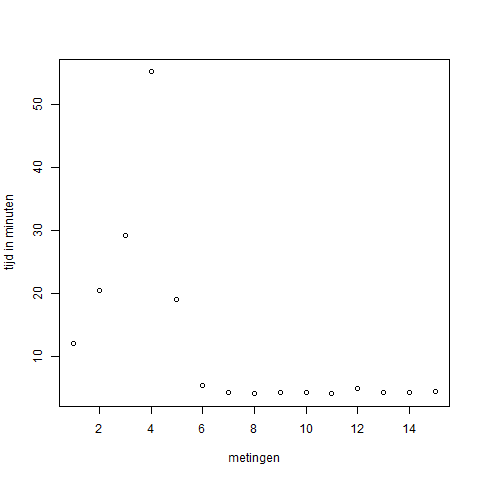
\includegraphics[scale=0.5]{img/centosplotfull.png}
\end{center}

%% boxplot
\begin{center}
	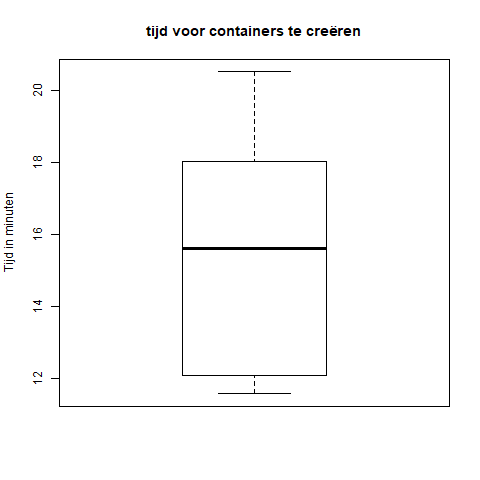
\includegraphics[scale=0.5]{img/centosboxplotfull.png}
\end{center}

%% gemiddelde
$\mu = 12.06457$

%% variantie
$\sigma^2 = 203.7204$

%% standaarddeviatie
$\sigma = 14.27307$

De gemiddelde benodigde tijd voor het commando bij de CentOS-opstelling was laag en vrijwel stabiel, met maar een paar outliers. De reden voor deze outliers kwam omdat deze metingen genomen waren in een omgeving met een slechtere internetverbinding.

Dit was dus de grootste bottleneck voor deze opstelling. De impact hiervan op de installatie was in dit geval groot, zoals te zien valt aan de hoge variatie en standaarddeviatie.

Maar, in het algemeen valt was de performantie van de CentOS-opstelling goed te noemen.

\subsection{Performantie containers}
Vervolgens kan men hier de resultaten zien voor elke keer dat het 'time vagrant provision'-commando werd uitgevoerd op de CentOS-opstelling. Deze keer uitgedrukt in seconden.

Bij deze resultaten moest het Operating System niet meer geïnstalleerd worden en ook de Docker Image moeten niet meer gedownload worden. Er werd alleen gekeken hoelang de Docker Daemon nodig had om de orders te interpreteren en de container tot staand te brengen.

%% plot
\begin{center}
	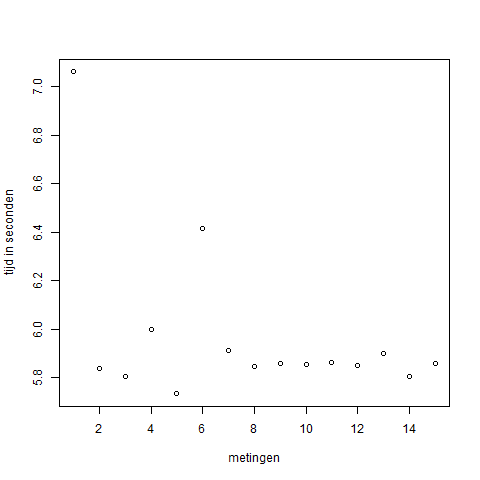
\includegraphics[scale=0.5]{img/centosplotprovision.png}
\end{center}

%% boxplot
\begin{center}
	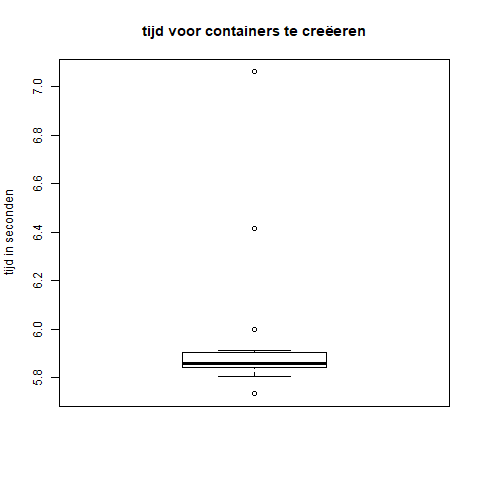
\includegraphics[scale=0.5]{img/centosboxplotprovision.png}
\end{center}

%% gemiddelde
$\mu = 5.972333$

%% variantie
$\sigma^2 = 0.1150491$

%% standaarddeviatie
$\sigma = 0.3391889$

De installatie van alleen de container ging vlot, met een stabielere gemiddelde tijd, en een kleinere variantie en standaarddeviatie. Dit kwam doordat de applicaties en Docker Images niet meer gedownload diende te worden. Hierdoor lagen de tijden veel lager en was er geen invloed meer van de bottleneck.

\section{Windows Server 2016}
\subsection{Performantie installatie}
Vervolgens kan men ook de resultaten zien van 'time vagrant up' voor de Windows-opstelling.

%% plot
\begin{center}
	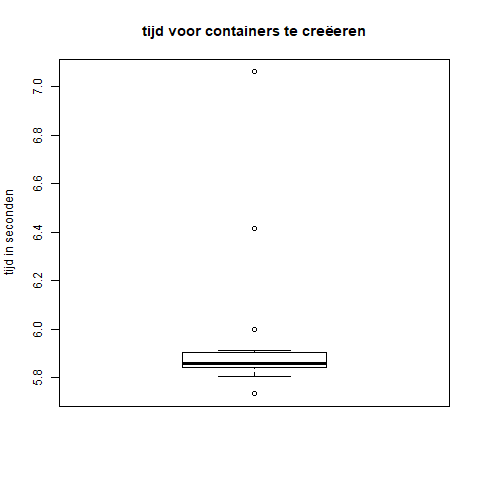
\includegraphics[scale=0.5]{img/centosboxplotprovision.png}
\end{center}

%% boxplot
\begin{center}
	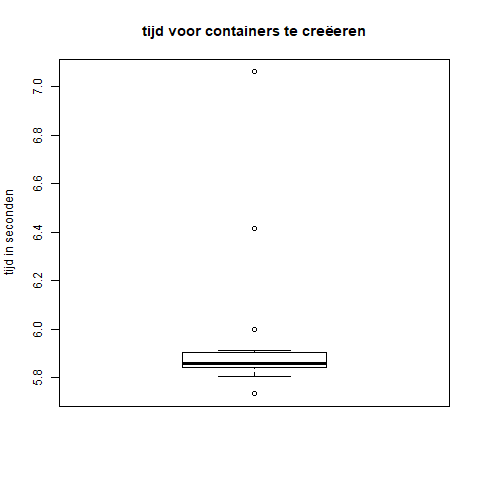
\includegraphics[scale=0.5]{img/centosboxplotprovision.png}
\end{center}

%% gemiddelde
$\mu = 5.972333$

%% variantie
$\sigma^2 = 0.1150491$

%% standaarddeviatie
$\sigma = 0.3391889$

De installatie van de Windows opstelling duurde gemiddeld 10 keer langer dan de centOS-opstelling. De gemiddelde tijd voor een volledige installatie was immers 45 minuten. De variantie en standaarddeviatie lagen ook . Hier waren verschillende redenen voor:

\begin{itemize}[noitemsep]
	\item Installatie Windows OS
\end{itemize}

Om te beginnen duurde de installatie van het besturingssysteem langer omdat er een GUI gebruikt werd. Als Windows Server Core werd gebruikt zou de performantie al sterk verbeteren. Maar, dan kon men geen Docker CE for Windows installeren. Windows Server Nano was helaas ook geen optie, omdat deze helemaal niet ondersteund werd door Docker for Windows, zelfs niet voor Docker EE. Ten slotte hoefde CentOS ook niet heropgestart te worden na de installatie van Docker.

\begin{itemize}[noitemsep]
	\item Microsoft SQL server container
\end{itemize}

De MSSQL server container voor Windows was meer dan 10 keer zo groot als de Linux variant,  6GBs tegenover 479MBs. Hierdoor was de installatie een groot deel van zijn tijd bezig met het downloaden van deze Docker Image.

\subsection{Performantie applicatie}
Ten slotte kan men hieronder ook de resultaten zien van 'time vagrant provision' voor de Windows-opstelling van alleen de benodigde tijd om de containers te installeren.

%% plot
\begin{center}
	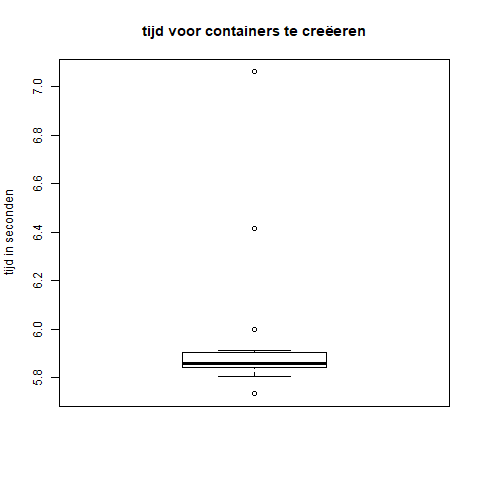
\includegraphics[scale=0.5]{img/centosboxplotprovision.png}
\end{center}

%% boxplot
\begin{center}
	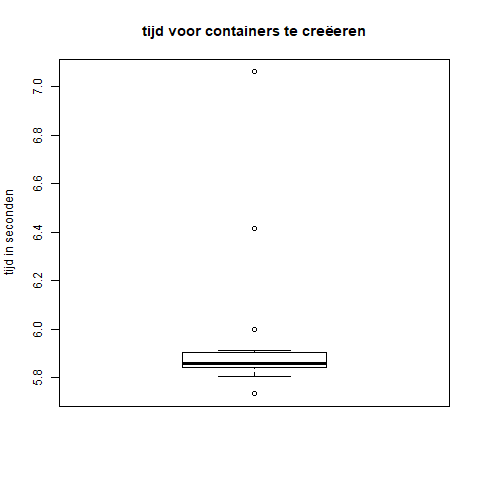
\includegraphics[scale=0.5]{img/centosboxplotprovision.png}
\end{center}

%% gemiddelde
$\mu = 5.972333$

%% variantie
$\sigma^2 = 0.1150491$

%% standaarddeviatie
$\sigma = 0.3391889$

Hier waren de resultaten al iets meer gelijk aan de CentOS-opstelling. Doordat de Windows-opstelling nu niet meer tijd verloor met het installeren van een GUI, heropstarten of downloaden van grotere Docker Images.

\section{Conclusie}

%%=============================================================================
%% Securitytest
%%=============================================================================

\chapter{Security test}
\label{ch:securitytest}

Dit hoofdstuk vergelijkt de verschillende manieren waarop beide besturingssystemen, Linux en Windows, in staat zijn om hun systemen te beschermen. Deze security review vergelijkt welke industriestandaarden beide systemen kunnen implementeren om hun systemen te harden tegen aanvallen.

Zoals eerder gezegd is een container automatisch veiliger dan een klassieke VM, omdat er een isolatielaag ligt tussen de container en het besturingssysteem waarop het draait. Echter, als men toch via de container toegang zou kunnen verkrijgen tot het host-systeem, wat dan? Elk systeem is namelijk even sterk als zijn zwakste schakel. Dit werd ook bevestigd voor Solomon Hykes, CTO van Docker op DockerCon 2017 in Austin, USA op vlak van Linux beveiliging. Hij zei: "We denken dat Docker niet de verantwoordelijkheid is om Linux subsystemen te beveiligen. Sterker nog, we denken niet dat deze verantwoordelijkheid bij één bedrijf in het bijzonder moet liggen. Linux is té groot en té belangrijk, dus daarom is het zó belangrijk dat veiligheid vanuit de community komt. En de community is goed bezig: iedereen werkt samen, in plaats van elk in zijn eigen hoekje".

Daarom zal deze security review vertrekken vanuit de populairste veiligheidsopties voor het harden van een CentOS machine, waarna deze vergeleken zullen worden met equivalente opties voor Windows.

\section{CentOS}
\subsection{Linux containers}
Als eerste werd er gekeken naar hoe Linux-containers tot staande gebracht worden en hoe sterk het isolatieniveau ervan is.

Zoals in de inleiding reeds vermeld hebben Linux-containers hun eigen netwerk resources, geheugen, geïsoleerde CPU en I/O block, maar maken ze wel gebruik van dezelfde kernel als het host besturingssysteem. Dit zorgt ervoor dat containers licht en gestroomlijnd kunnen zijn, maar dit kan zorgen voor zowel sterktes als zwaktes.

Om te beginnen is het veel moeilijker om diepe toegang te krijgen tot de hoogst mogelijke privileges bij een container. Dit is een direct gevolg van de isolatie tussen de container en zijn host. Echter, als dit wel lukt, is er een reëel probleem. De Linux Container deelt immers de kernel met zijn host-systeem, waardoor system calls een groot probleem vormen. Door een geminimaliseerde OS te gebruiken kan men dit probleem verminderen, maar niet verhelpen.

Daarnaast is er wel het voordeel dat Root-toegang tot de container niet automatisch betekent dat men Root-toegang heeft op het host-systeem, maar dan moet men wel oppassen voor privileged containers. Deze worden namelijk wel standaard gebonden aan het host uid 0, waardoor deze containers niet root-safe zijn en ook niet root-safe gemaakt kunnen worden. Daarom maakt men best gebruik van Mandatory Access Control, zoals SELinux of AppArmor, seccomp filters en het laten vallen van namespaces.

Vervolgens is er het probleem dat Cgroups standaard geen limiet heeft, waardoor men gemakkelijk een Denial of Service-attack kan uitvoeren op een CentOS-systeem. Dit risico kan verlaagd worden door memory, cpu en pods aan te passen in de configuratie van lxc.cgroup.

Ten slotte zijn aanvallers vaak teleurgesteld als ze in een container geraken, want best practice zegt "geen data in containers", waardoor de voornaamste aanvalreden niet veel zal opleveren. Kijk maar naar de ransomware attacks die steeds populairder worden. Deze hebben als doel om data 'gevangen' te nemen tot het losgeld ervoor betaald is. \autocite{Weissig2013 } \autocite{Reno2016} \autocite{Wang2017}

\subsection{SELinux}
SELinux of Security-Enhanced Linux gebruikt Linux Security Modules (LSM) om een Linux-systeem te harden tegen aanvallen. De verschillende modules kunnen worden aan- of uitgezet via een reeks van booleans. Daarnaast kan men ook handgemaakte waardes toevoegen aan deze lijst om ze te blokkeren of door te laten.

SELinux bestaat uit onderwerpen, zoals users of applicatieprocessen. Daarnaast bestaat het uit objecten, zoals bestanden en folders, en uit een set van regels. Deze regels bepalen wat een onderwerp mag doen met een object.

Voor Docker bestaat er ook een SEModule. Deze module moet eerst enabled worden via 'semodule -v -e docker'. Daarna dient Docker te worden herstart met de volgende waarde: --selinux-enabled. Deze waarde dient te worden geplaatst in docker.service configuratiebestand. Ten slotte dient men Docker opnieuw op te starten, waarna Docker altijd met SELinux enabled zal opstarten.

De invloed van deze module is veelvoudig. Het belangrijkste gevolg is dat men kan beperken tot welke folders Docker toegang heeft, want de 'privileged' Docker-processen krijgen niet dezelfde privileges als andere privileged processen. Daarnaast kan men via het 'docker run'-commando de kernel-mogelijkheden beperken door er '--cap-drop=' aan toe te voegen.

Van alle tools die beschikbaar zijn om een Linux-server te beveiligen, is SELinux veruit de krachtigste. Het grootste nadeel bij SELinux is echter dat de gebruiksvriendelijkheid niet evident is; het is een moeilijke tool. Ondanks dit nadeel loont het wel om vaardig te worden binnen deze module. \autocite{Henry-Stocker2012} \autocite{Juggery2017} \autocite{Walsh2013}

\subsection{Firewalld}
Daarnaast kan men op CentOS Firewalld configureren om bepaalde poorten te openen of te blokkeren. In essentie gebruikt Firewalld gewoon IpTables met een XML-overlay, wat het gebruik ervan veel vergemakkelijkt heeft. Hiermee kan men de verschillende zones en poorten instellen die men wil blokkeren of doorlaten, maar men kan ook gekende services toevoegen aan Firewalld, waarbij deze automatisch de standaardpoorten ervoor opent of sluit. Standaard is de zone 'public' en worden de meeste poorten geblokkeerd. \autocite{Brown2014} 

\subsection{Seccomp}
Ten slotte kan men ook Secure Computing gebruiken (Seccomp) gebruiken. Hiermee kan men de system calls beperken die een process kan maken. Hierdoor kan het systeem beschermd worden tegen hackers, wanneer ze system calls willen maken die niet eerder gedeclareerd zijn. Hoewel Seccomp in het verleden stroef was om te gebruiken, is het gebruik (Libseccomp) ervan sterk gegroeid, onder andere door de toevoeging van BPF (Berkeley Packet Filters). BPF werd in het verleden gebruikt om netwerk pakketten te filteren, maar door het potentieel ervan groeiden de toepassingen ervoor ook.

Seccomp's voordelen liggen vooral in het blokkeren van system calls vanuit de containers naar het host-systeem, als deze niet van toepassingen zijn. Daardoor kunnen aanvallen vanuit de container end-points tegengehouden worden. \autocite{Arora2012} \autocite{Spijkers2013}

\section{Windows}
\section{Hyper-V containers}
Hyper-V Containers, zoals die gebruikt worden door Docker for Windows, verschillen op één belangrijke manier van Linux Containers. Hyper-V containers gebruiken namelijk de base image om een VM aan te maken, door deze in de Hyper-V partition wrapper te steken, waarna er in deze VM een Windows-container wordt aangemaakt om de applicatie in te steken. Hierdoor is er een extra isolatielaag tussen de container en de kernel, namelijk de Hypervisor van de VM. Dit verhelpt veel van de problemen die de Linux Containers hebben op vlak van kwetsbaarheden.

Hier staat echter wel een kost tegenover. Dit zorgt er namelijk voor dat de Hyper-V containers in het algemeen groter zullen zijn dan Linux Containers, en dat ze meer tijd zullen nodig hebben om opgezet te worden. De last is gelukkig niet al te groot, aangezien Hyper-V een type 1 Hypervisor is en dus rechtstreeks op de hardware draait. Ten slotte bestaat er ook het gevaar dat de VM crasht wanneer men in de container zit, waardoor men niet meer uit de container boundaries zal geraken. \autocite{Savill2015}

\section{Integrity levels}
Windows Integrity Checks (WIC) is het Windows-equivalent van SELinux. Deze functie zat reeds ingebouwd in Windows Vista, waar het als doel had om objecten te beschermen, zoals bestanden, printers en pipes. WIC werkt door de betrouwbaarheid van alle objecten en de interactie hiermee een waarde te geven, zogezegd een level of trustworthiness. Als men een actie wil uitvoeren op dit object, zal men het niveau op zijn minst moeten evenaren. WIC heeft een grotere prioriteit dan normale permissies.

Er zijn in totaal zes niveaus die WIC kan geven aan objecten. Van laag naar hoog zijn dit:

\begin{itemize}[noitemsep]
	\item untrusted (anonieme processen)
	\item low (interactie met het internet)
	\item medium (meeste objecten, onder andere de shell)
	\item high (Administrators)
	\item system (system)
	\item installer (speciaal voor .EXE's)
\end{itemize}

Hoewel deze functie praktisch onopgemerkt is gebleven, heeft dit de veiligheid van Windows wel sterk verbeterd. Hiervoor had Windows namelijk geen enkele manier om aan Mandatory Access Control te doen. Helaas is er wel nog werk aan de winkel. Er is bijvoorbeeld een gebrek aan management of een configuratietool voor administrators. Daarnaast is het systeem ook niet feilloos, zoals er in Vyacheslav Rusakov wordt aangetoond. \autocite{Khanse2009} \autocite{Bradley2007} \autocite{Rusakov2016}

\section{Windows Defender}
Windows Defender is begonnen als een anti-spyware systeem, waarnaast men nog andere antivirus-functies moest installeren, zoals Microsoft Security Essentials, om een complete verdediging te hebben. Sinds Windows 8 heeft het echter ook definitief deze rol overgenomen.

Qua performantie krijgt Windows Defender gemengde reviews. Vooral de firewall van Windows Defender kan een last vormen op de CPU. Daardoor is de meest gezochte term voor Windows Defender hoe je het uitschakelt. Vaak is het beter om een extra third-party systeem te gebruiken voor de firewall, zoals een PFSense of een WatchGuard. \autocite{Hall2017} \autocite{Lefferts2017}

\subsection{ACL}
Het Windows-equivalent voor Seccomp is Windows Access Control Lists. De ACL bestaat uit een lijst van Access Control Entries (ACE's), waarbij elke ACE een trustee aanduidt en bepaalt welke Access Rights deze heeft. Helaas wordt het niet aangeraden om rechtstreeks met de inhoud van een ACL te werken. Er zijn functies en modules om deze te wijzigen, maar ook hier kan de administrator geen rechtstreekse invloed hebben op het systeem. \autocite{Rapid72017}

\section{Conclusie}
Linux heeft een meer hands-on aanpak om zijn systemen te beveiligen, waarbij de administrator van het Linux-systeem veel zelf kan en moet bepalen. Dit betekent wel dat de veiligheid van een Linux-opstelling even goed is als de kennis van zijn administrator, wat zowel positief als negatief kan zijn. Windows daarentegen neemt veel controle van de administrator weg, en doet het werk voor hem. Dit betekent dat er een basisniveau is qua veiligheid, maar dat dit niveau ver onder het niveau van een Linux-opstelling kan liggen, vooral als de administrator reeds veel kennis verworven heeft.
%%=============================================================================
%% Conclusie
%%=============================================================================

\chapter{Conclusie}
\label{ch:conclusie}

%% TODO: Trek een duidelijke conclusie, in de vorm van een antwoord op de
%% onderzoeksvra(a)g(en). Wat was jouw bijdrage aan het onderzoeksdomein en
%% hoe biedt dit meerwaarde aan het vakgebied/doelgroep? Reflecteer kritisch
%% over het resultaat. Had je deze uitkomst verwacht? Zijn er zaken die nog
%% niet duidelijk zijn? Heeft het onderzoek geleid tot nieuwe vragen die
%% uitnodigen tot verder onderzoek?

%%Inleiding
De onderzoeksvraag voor deze bachelorproef was: hoe goed presteert Docker for Windows op vlak van performantie en veiligheid tegenover Docker for Linux? Hiervoor werden er twee systemen opgesteld. Waarbij de eerste opstelling een Windows Server 2016 met Docker for Windows is. De tweede opstelling bevatte een CentOS 7.4 met Docker for Linux. Vervolgens werd de performantie van beide systemen vergeleken door te kijken hoe lang beide nodig hadden om een volledige installatie uit te voeren en hoeveel tijd voor alleen hun containers. Ten slotte werd de beveiliging van beide systemen onder de loop genomen. Waarbij er vertrokken werd uit de veiligheidsmaatregelen die men kan nemen met CentOS en of Windows hier een equivalent voor had. 

%%Concrete resultaten/cijfers van Docker for Windows voor DevOps
%%Performantie
Welk systeem de betere performantie had was duidelijk. Bij de volledige installatie had Windows tot wel 10 keer meer tijd nodig om alles geïnstalleerd te krijgen. Dit komt onder andere doordat Docker for Windows een GUI nodig heeft om te installeren. Daarnaast zijn de containers en base images groter dan die voor Linux. Dit zijn twee hekelpunten die zeker nog weggewerkt moeten worden door Docker en Microsoft. Zeker als men Docker for Windows ook verkocht wilt krijgen aan DevOps teams.

Aan de andere kant, deze grafische interface maakt Docker wel veel toegankelijker voor beginnende developers die op een Windows OS werken. Deze hebben immers geen nood aan een volledig geautomatiseerde omgeving. Maar, hechten veel meer waarde aan een toegankelijke applicatie. Daarnaast zijn deze developers niet meer verplicht om een Linux VM te draaien op hun systeem. Ten slotte, zullen deze beginnende developers ook niet evenveel containers draaien als een professionele onderneming. Waardoor de grote ervan minder belangrijk is.

Mijn conclusie voor performantie is dat Docker for Linux meer geschikt zal zijn voor bedrijven die op een professionele manier willen omgaan met container-technologie. Maar, dat Docker for Windows meer geschikt is voor beginnende developers. Zeker als men al werkt op een Windows systeem.

%%Veiligheid
Op vlak van veiligheid ligt de bal een beetje meer in het midden. Linux heeft enkele sterke voordelen, zoals SELinux, Firewalld en Seccomp. Maar, dit vereist wel enige kennis. Dus, is de beveiliging van Linux voor een groot deel afhankelijk van de kennis van zijn administrator. Daartegenover is de beveiliging van Windows veel meer basic. Maar, is er wel een minimum aan veiligheid doordat Microsoft bepaalde beslissingen uit de handen van zijn administrators neemt en deze instelt voor hem. Dit is zowel een voor- als nadeel. Want ook Microsoft is niet feilloos. Maar, Hyper-V Containers zijn dan wel weer een pak veiliger dan de Linux Containers. Doordat ze een extra niveau van isolatie hebben.

%%Resultaat werk
%%Nee, Windows veel trager.
De resultaten van dit onderzoek zijn min of meer binnen de lijnen van het verwachte. Alleen de performantie kun je vrij schokkend noemen. Als Docker en Microsoft Docker for Windows even competitief willen maken als Docker for Linux is er nog werk aan de winkel. Op vlak van veiligheid zijn beide systemen equivalent aan elkaar. Waar vooral de kennis van de administrator een grote rol speelt.

%%Veiligheid kan verder uitgebreid worden
%%PowerShell en Docker
%%Hoe verder automatiseren van Docker for Windows en beter
Verdere onderzoeksvragen die uit deze bachelorproef oprijzen zijn:
\begin{itemize}[noitemsep]
	\item Hoe goed integreert Docker for Linux met het Windows besturingssysteem?
	\item Kun je de installatie van Docker for Windows beter automatiseren door PowerShell modules aan te maken?
	\item Zijn er manier om de grote van de Hyper-V containers te verkleinen?
\end{itemize}

\appendix

%%---------- Back matter ------------------------------------------------------
\printbibliography
\addcontentsline{toc}{chapter}{\textcolor{maincolor}{\IfLanguageName{dutch}{Bibliografie}{Bibliography}}}


\listoffigures
\listoftables

\end{document}
